\documentclass[Japanese]{dicomopapers}
%\documentclass[Japanese,noauthor]{dicomopapers}

\usepackage[dvips]{graphicx}
\usepackage{latexsym}

\def\Underline{\setbox0\hbox\bgroup\let\\\endUnderline}
\def\endUnderline{\vphantom{y}\egroup\smash{\underline{\box0}}\\}
\def\|{\verb|}

\begin{document}

% 和文表題
\title{IoTデバイスの通信セキュリティ向上のための\\ホームネットワーク仮想化フレームワークの提案}
% 英文表題
\etitle{Proposal of Home Network Virtualization Framework\\to Improve Communication Security of IoT Devices}

% 所属ラベルの定義
\affiliate{DOSHISHA}{同志社大学大学院 理工学研究科\\Graduate School of Science and Engineering, Doshisha University}
\affiliate{MOBILITY}{同志社大学モビリティ研究センター\\Mobility Reserch Center, Doshisha University}

\author{塚崎 拓真}{TAKUMA TSUKASAKI}{DOSHISHA}
\author{滕 睿}{RUI TENG}{MOBILITY}
\author{佐藤 健哉}{KENYA SATO}{DOSHISHA}

\begin{abstract}
	近年,IoT(Internet of Things)が注目を集めるようになり,今後あらゆるモノがネットワークに接続され,利用されることが予想される.しかし,IoTの発展により利便性が高まる一方で,これまでネットワークに接続されていなかったモノが接続されることにより,セキュリティ上のリスクも高まっている.また,今後はホームネットワーク内で閉じたデバイス間の通信によって連携を行う形になることが想定される.デバイス間で直接通信を行う場合,各デバイスにおいてアクセス制御等の更なるセキュリティ対策を行う必要がある.そこで本研究では,各IoTデバイスに柔軟にセキュリティ対策を適用するために,コンテナを用いてIoTデバイス間通信を中継することで,各デバイスに対してセキュリティ対策を適用できるシステムを提案した.また,ホームネットワーク内の通信のトラフィック情報は既知であるため,提案システムではOpenFlowを用いて,ホームネットワーク内の通信を監視するフレームワークの構築も検討した.そして,IoTデバイス間で閉じた通信を行うシミュレーションの評価を行い,ホームネットワークにおいてセキュリティ要件を保つことを示した.
\end{abstract}

% 表題などの出力
\maketitle

% 本文はここから始まる
\section{はじめに}
近年,IoT(Internet of Things)の可能性が注目され,今後あらゆるモノがネットワークに接続され,利用されることが予想される.
あらゆるモノがネットワークに接続されることで,ビッグデータを収集し,活用することが可能となる.また,ローカルネットワーク内においても,様々なIoTデバイスの普及により,従来,相互接続されていなかった機器同士の接続が想定される.このような変化により,生活や産業の効率・利便性を高めることが期待されている.\par
しかし,IoTの発展により利便性が高まる一方で,従来ネットワークに接続されていなかったモノが接続されることにより,セキュリティ上のリスクも高まっている\cite{security}.
IoTデバイスは,十分なセキュリティを考慮せずに開発されたものが多く,脆弱なパスワードによる侵入やプライバシー保護の不十分さ等のセキュリティ対策不足が顕著である\cite{owasp}.そのため,悪意のある攻撃者によるサイバー攻撃の標的になりやすい.
脅威としては,ホームネットワークに侵入し,デバイスの遠隔操作による外部サーバへの攻撃や,マルウェア感染によるプライバシーに関わる機密情報の収集などが挙げられる.
また,攻撃によってホームネットワーク内に侵入された場合,その内部においてもデバイス間で自由にアクセスできるため,マルウェア感染などのリスクがホームネットワーク全体のデバイスに広がる可能性がある.そのため,ホームネットワークのセキュリティ対策として,内部への侵入を前提に,攻撃を受けた際に被害を最小化することが重要である.\par
しかし,IoTデバイスは従来のPC等の既存機器と比較した場合,CPU等のリソースを十分に保持していない\cite{camera}ため,デバイスの計算能力の制限やソフトウェア自体の脆弱性によって,適用できる機能が限られるという問題がある\cite{disap}.
そのため,暗号化等のセキュリティ対策の適用は困難となり,全デバイスが接続するネットワークを利用したシステムを構築することや,仮想的にセキュリティ対策を施し,デバイスのリソース制限に捉われないシステムを構築することが望ましい.\par
そこで本研究では,コンテナ上にセキュリティ対策を施したProxyを作成し,IoTデバイスに対してセキュリティ対策を適用するシステムを提案する.また,SDN(Software Defined Networks)の代表的プロトコルであるOpenFlow\cite{openflow}を用いて,ホームネットワーク内の通信を監視するフレームワークの構築も検討する.


% \section{ホームネットワークの問題点}
% IoTデバイスが普及し,スマートホーム等の考えが生まれると,アンチウイルスソフトやファイアウォール等のエンドポイントにおけるセキュリティ対策だけでは困難である.これは,カメラやスマート家電等のIoTデバイスでは,処理能力が低く,エンドポイントセキュリティ対策に求められる要件を満たさないためである\cite{camera}.さらに,独自に組み込み用OSが使われているものもあり,それら全てに対応したシステムの構築や更新を続けると非常にコストが高くなる.
% そのような状況の中,脆弱なパスワードでの侵入やデータのプライバシー保護が不十分であることや,安全でないデータの転送等のIoTデバイスのセキュリティ対策不足が顕著になる\cite{owasp}.
% 上記の脆弱性から,IoTデバイスが他のデバイスへの感染や攻撃に悪用され,侵入や感染などの被害によってデータ流出や外部サービスへの攻撃などの恐れがあるため,侵入を前提に考えなければならない.このことから,ホームネットワークセキュリティ対策として必要なことは,侵入感染後の被害の最小化である.


\section{関連研究}
\subsection{フローレベルの攻撃検知・防止}
Sivanathanらは,SDNと外部の解析エンジンを用いて,IoTデバイスのネットワークを常に監視し,フローレベルでのトラフィック検査を行う手法を提案した\cite{lowcost}.IPアドレスやポート番号等のフロー情報から攻撃を検知できることを示し,パケットベースのネットワーク監視と比較し,処理コストの大幅な削減を実現した.\par
しかし,ホームネットワーク内のトラフィック情報検査を外部で行っていることが問題点として挙げられる.今後のIoTデバイスは,ホームネットワーク内で閉じたデバイス間の通信によって,相互の連携を行う形になることが想定される\cite{d2d}.デバイス間で直接通信を行う場合,各デバイスにおいてアクセス制御等のセキュリティ対策を行う必要がある.


\subsection{ホームネットワーク運用の外部依存を避けた自己完結型システム}
Zhangらは,クラウド上の遠隔サーバから制御されている現状のホームネットワークの問題点を挙げ,IoTデバイスの管理をクラウドや外部サービスに依存しないホームネットワークシステムを提案した\cite{sover}.トラストアンカーをローカルコントローラに置くことで,デバイスやアプリケーションの管理や,データ検索等の承認,制御をホームネットワークシステム内で行うことを可能にした.その結果,クラウドを用いたシステムより,遅延を低減した.\par
しかし,各IoTデバイスに対応したセキュリティ対策を施す柔軟性を持ち合わせていない.ホームネットワーク内には,異なる規格のハードウェアや様々なアプリケーションが混在しているため,各デバイスに対して柔軟にセキュリティ対策を適用できるシステムを構築することが望ましい.

\begin{figure}[!tb]
	\centering
	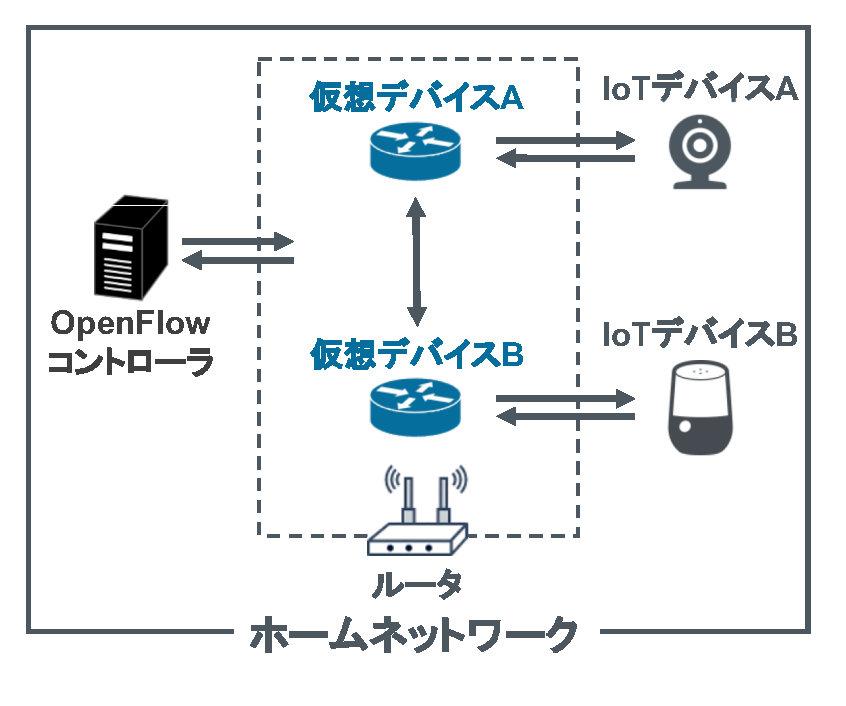
\includegraphics[width=\linewidth]{img/system.eps}
	\caption{提案システムの構成}
	\label{fig:system}
\end{figure}


\section{提案システム}
\subsection{概要}
本研究では,コンテナ上にセキュリティ対策を施したProxyを作成し,IoTデバイスに対してセキュリティ対策を適用するシステムを提案する.提案システムでは,IoTデバイスがリソース量の制限により適用できないセキュリティ対策をProxyにオフロードする.そして,IoTデバイス間の通信を中継することで,本来IoTデバイスに適用したいセキュリティ対策を実現する.
また,OpenFlowの機能も追加し,ネットワークの監視を行う.ホームネットワーク内通信のトラフィック情報は既知であることを考慮し,フローの検証をOpenFlowコントローラで行う.
詳細なセキュリティ対策については後述する.


\subsection{システム構成}
提案システムの構成を図\ref{fig:system}に示し,詳細を以下に示す.本提案システムは,IoTデバイス,Proxy,ルータ,OpenFlowコントローラから構成される.
\begin{itemize}
	\item \underline{IoTデバイス}\mbox{}\\
	      本研究で扱うIoTデバイスは,CPU等のリソースを十分に保持しておらず,直接セキュリティ対策を適用できないデバイスと定義する.
	\item \underline{Proxy}\mbox{}\\
	      IoTデバイスに要求されるセキュリティ対策を,コンテナ上で実現したものである.そして,IoTデバイスからの通信を中継し,セキュリティ対策を適用する.各IoTデバイスに必要なセキュリティ対策をそれぞれ作成,適用することで,対象デバイスに応じた必要なセキュリティ対策を実現できる.
	\item \underline{ルータ}\mbox{}\\
	      IoTデバイス間通信の中継機器として用いる.ルータ上にProxyの実行環境を生成する.Proxyが作成される際に必要とされるリソースを提供することが可能である.
	\item \underline{OpenFlowコントローラ}\mbox{}\\
	      Proxy内に作成されたOpenFlowスイッチと通信を行い,ホームネットワーク内の通信を監視する.ホームネットワーク内部に設置する.
\end{itemize}

\begin{figure}[!tb]
	\centering
	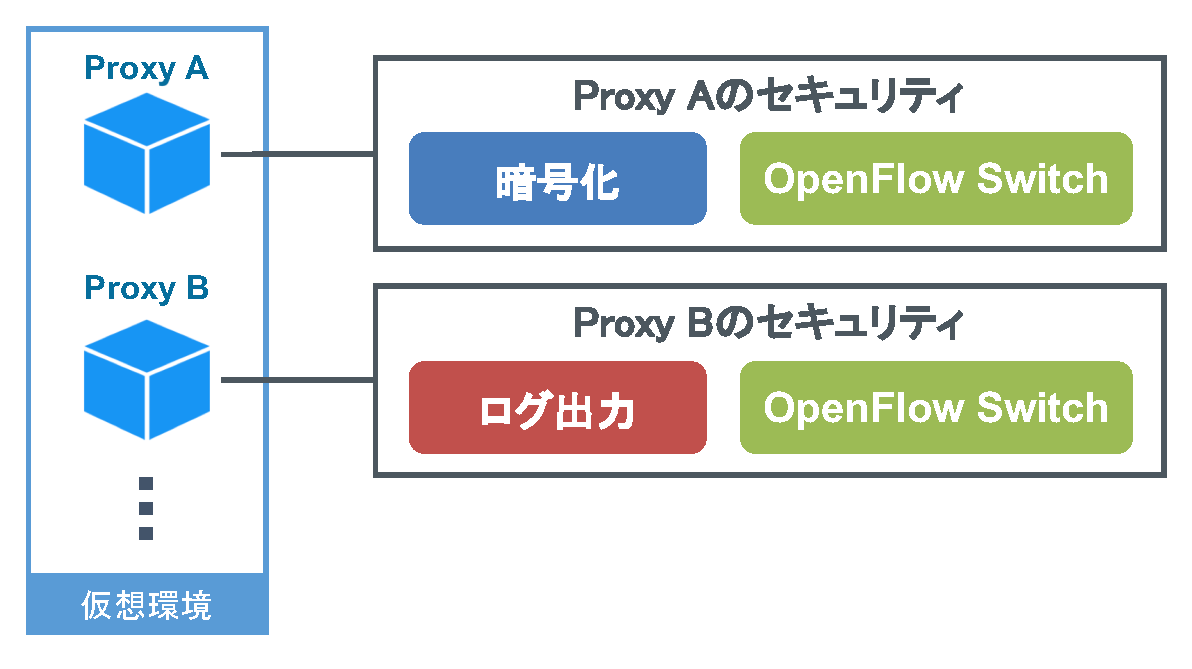
\includegraphics[width=\linewidth]{img/security.eps}
	\caption{Proxyのセキュリティ対策}
	\label{fig:security}
\end{figure}

\begin{figure}[!tb]
	\centering
	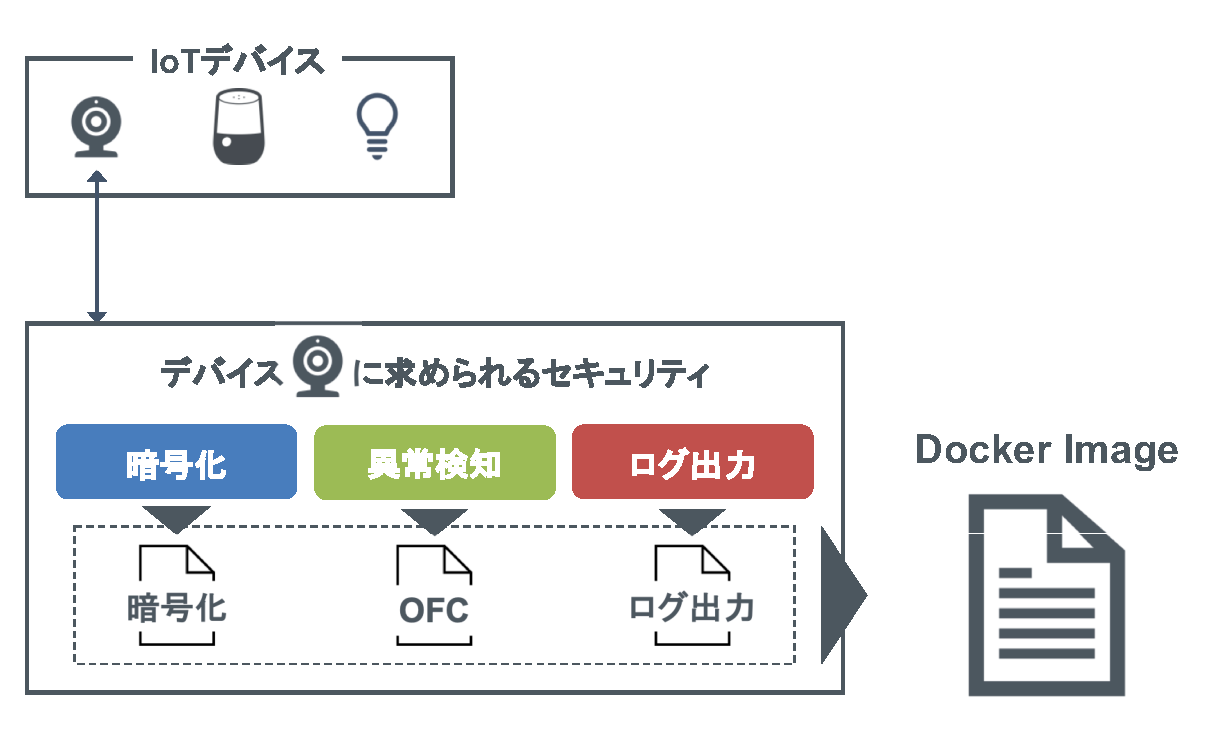
\includegraphics[width=\linewidth]{img/dockerimage.eps}
	\caption{imageファイルの作成}
	\label{fig:dockerimage}
\end{figure}

\subsection{Proxyのセキュリティ対策}
本研究におけるセキュリティ対策は,Proxyごとに異なるセキュリティ対策を適用可能である.Proxyのセキュリティ対策の適用例を図\ref{fig:security}に示す.これにより,リソース制限が原因でIoTデバイスに直接適用できないセキュリティ対策を適用できる.また,前述の問題点で述べたような様々なハードウェアやアプリケーションへの適用や,様々なセキュリティ要件の変更に対しても柔軟に対応が可能となる.\par
また,コンテナ上で作成されるセキュリティ対策は,各セキュリティ対策に対応したコンテナのimageファイルで定義される.imageファイルの作成例を図\ref{fig:dockerimage}に示す.IoTデバイスに適用したいセキュリティ対策が複数ある場合においても,対象デバイスの規格に対応したセキュリティ対策をそれぞれ作成し,ソフトウェアモジュールのような形で組み合わせて定義することで,imageファイルを作成することが可能となる.

\begin{figure}[!tb]
	\centering
	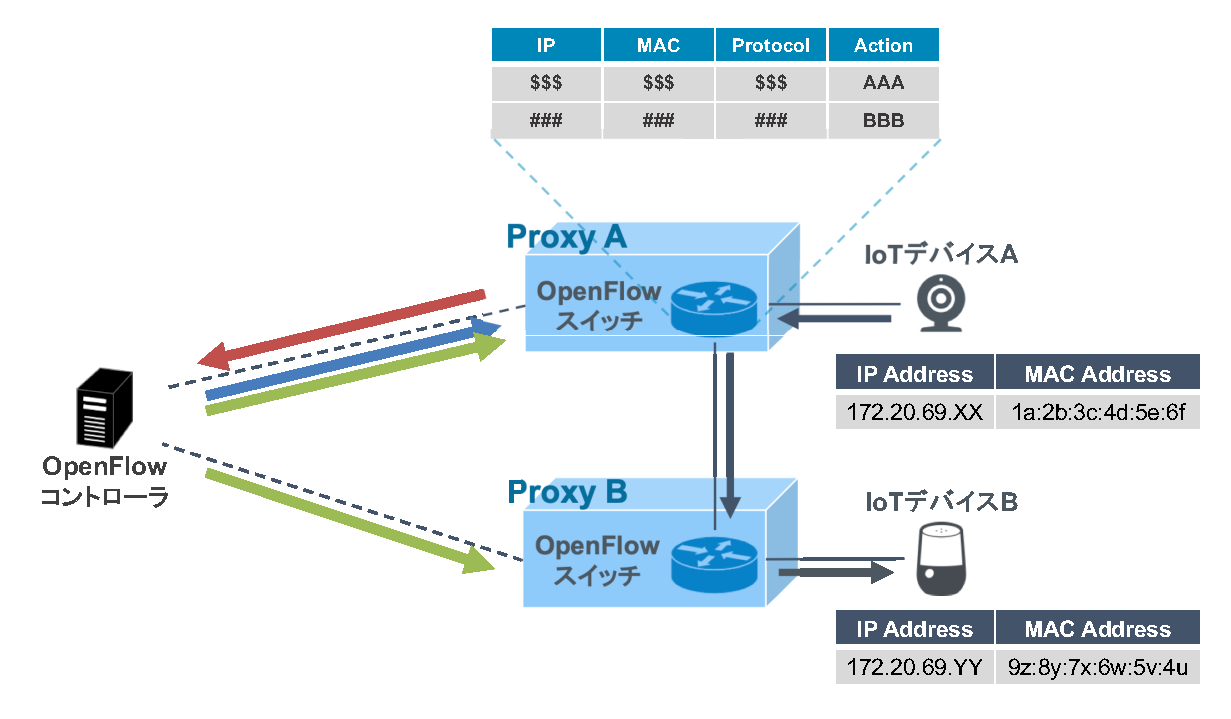
\includegraphics[width=\linewidth]{img/openflow.eps}
	\caption{OpenFlowにおけるフローチェック}
	\label{fig:openflow}
\end{figure}

\subsection{OpenFlowによるフローチェック}
本研究におけるネットワーク監視をOpenFlowを用いて行う.OpenFlowによるフローチェックを図\ref{fig:openflow}に示す.一つのIoTデバイスに対し,コンテナ上にOpenFlowスイッチの機能を生成する.IoTデバイスは,このOpenFlowスイッチを中継し,デバイス間通信を行う.OpenFlowコントローラは事前にIoTデバイスの情報を保持しており,OpenFlowスイッチとの通信が確立でき次第,デバイス間通信のフローテーブルを作成する.ホームネットワークの特性である各IoTデバイスのトラフィック情報は既知であることや,変化が大きくないことを考慮し,IPアドレスや通信頻度の確認を行い,フローレベルにおける異常の検知を行う.異常を検知した場合は,そのパケットのDrop処理を指示したフローテーブルに変更し,その後フローテーブルを削除する.また同時に,ユーザへ異常検知を通知する.

\begin{figure}[!tb]
	\centering
	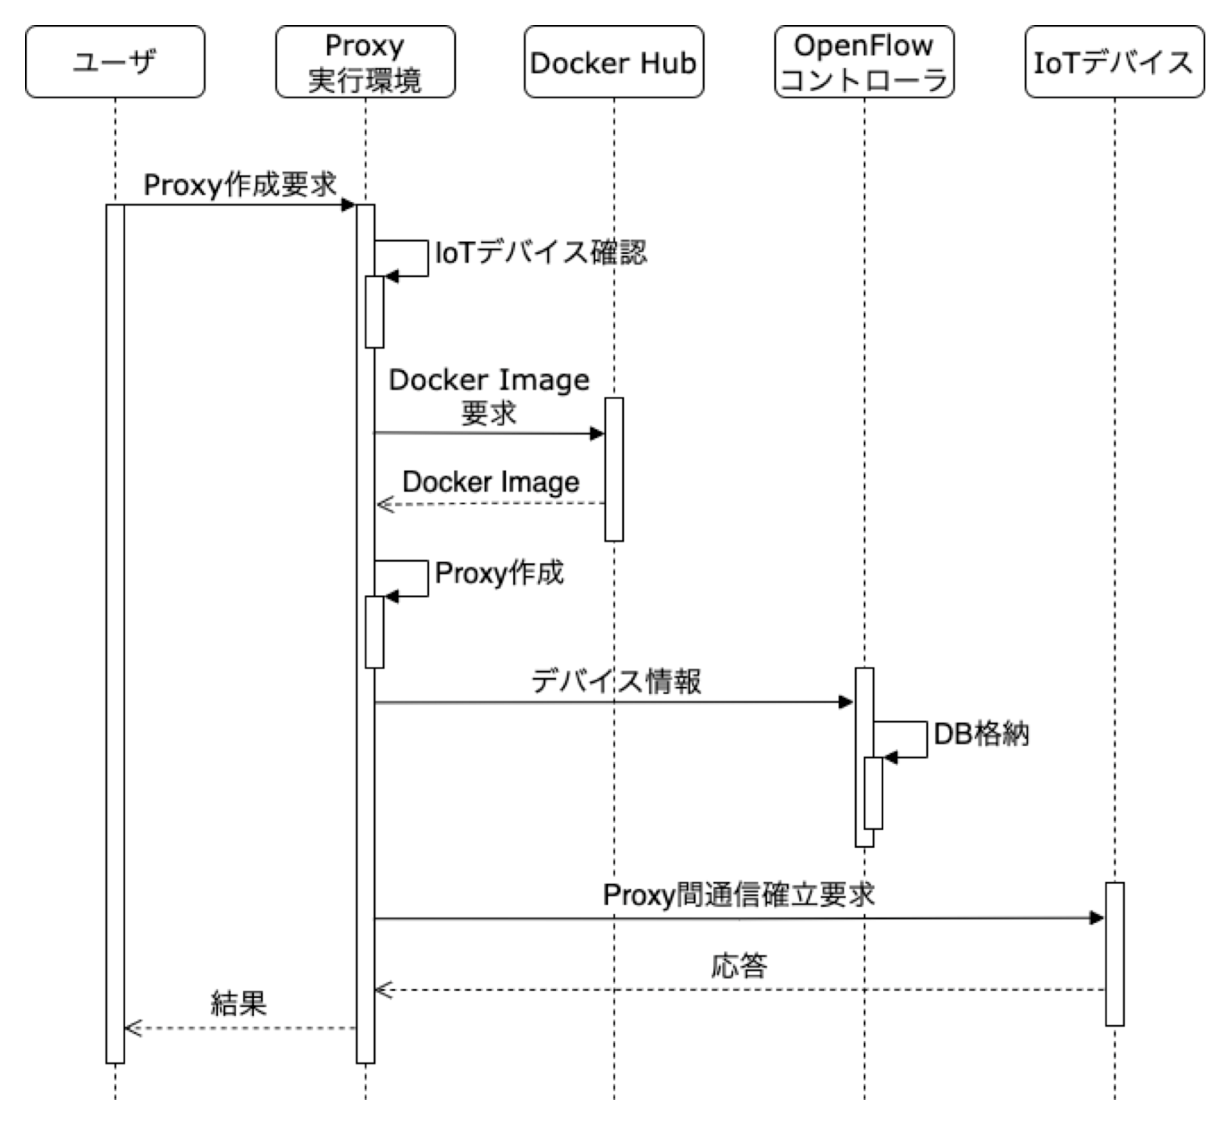
\includegraphics[width=\linewidth]{img/seaquence.eps}
	\caption{提案システムの動作手順のシーケンス図}
	\label{fig:seaquence}
\end{figure}

\subsection{動作手順}
本提案システムの動作手順を図\ref{fig:seaquence}に示し,詳細を以下に示す.
\begin{enumerate}
	\item ユーザは,デバイスをホームネットワークに接続した後,Proxyの実行環境へアクセスし,Proxyを作成するよう要求.
	\item 実行環境は,ホームネットワーク内にIoTデバイスが接続されたことを確認.
	\item 実行環境は,imageファイルのレジストリからimageファイルを取得.
	\item 取得したimageファイルを基に,実行環境内にProxyを作成.
	\item Proxyは,デバイス情報を基にIoTデバイスに接続を行い,Proxyを経由して通信を行うように設定.
	\item Proxyは,OpenFlowコントローラへデバイス情報を送信.
	\item 実行環境は,Proxyの設定が完了し,IoTデバイス・Proxy間の通信が確立された後,Proxyの作成・ネットワークの監視状況を報告.
\end{enumerate}


% \subsection{想定ユースケース}
% 本提案システムを用いた想定ユースケースを以下に示す.

% \begin{itemize}
% 	\item \underline{セキュリティ対策を事前に提供する場合}\mbox{}\\
% 	      SSL/TLSによる通信の暗号化など,IoTデバイスのリソース制限により適用できないセキュリティ対策を事前にimageファイルとして提供し,Proxy上で実現する.
% 	\item \underline{インシデント発生時などに対策を提供する場合}\mbox{}\\
% 	      事前に提供していたセキュリティ対策では想定していなかったインシデントが発生した場合に,対象デバイスが保持するリソース量に依存せず,追加のセキュリティ対策を提供することが可能となる.
% \end{itemize}

\begin{table}[!tb]
	\caption{実装環境}
	\label{tab:program}
	\centering
	\begin{tabular}{c|l|l}
		\hline
		種類                 & 項目       & 説明                  \\
		\hline \hline
		Proxy                & 使用ソフト & Docker                \\
		                     & OS         & Ubuntu 20.04          \\
		                     & CPU        & 3.60GHz Intel Core i9 \\
		                     & メモリ     & 5GB                   \\
		\hline
		OpenFlowコントローラ & 使用ソフト & Ryu                   \\
		                     & OS         & Ubuntu 20.04          \\
		                     & CPU        & 3.60GHz Intel Core i9 \\
		                     & メモリ     & 5GB                   \\
		                     & 使用言語   & Python                \\
		\hline
	\end{tabular}
\end{table}

\section{シミュレーション実験}
\subsection{実装環境}
本研究の実装に用いた環境を表\ref{tab:program}に,実装環境の構成を図\ref{fig:program}に示す.Proxyは,コンテナ仮想化を用いてアプリケーションを開発・実行するためのオープンプラットフォームであるDockerを用いて作成した.Dockerで作成されるコンテナ上でProxyを稼働させることで,複数のProxyをリソースやオーバーヘッドを抑えて作成できる.また,これらのProxyは,Docker Hubより配布されるDocker Imageを用いることで容易に作成でき,コンテナをアップロードして公開・共有できる.また,OpenFlowコントローラは,SDNを実現するための開発フレームワークであるRyuを用いて作成した.
% また今回扱う通信プロトコルとしてはhttp(REST)を想定する.

\subsection{評価内容}
本研究の評価として,まずセキュリティ対策が適用されているかを検証した.今回の異常通信としては,登録されていないIoTデバイスから通信があった場合と,あるデイバイスからの通信頻度が通常と異なる場合を想定した.その状況において,コンテナ上で作成したOpenFlowによるフローチェックが行われているかを検証した.\par
また,提案システムの有効性を示すため,提案システムを適用した上で,IoTデバイス間通信を行なった際のラウンドトリップタイムの計測を行った.比較対象として,セキュリティ対策を適用せず,ルータを経由してデバイス間通信を行う場合についても計測を行った.ラウンドトリップタイムは,20回通信を行なった際の平均値を算出した.

\begin{figure}[!tb]
	\centering
	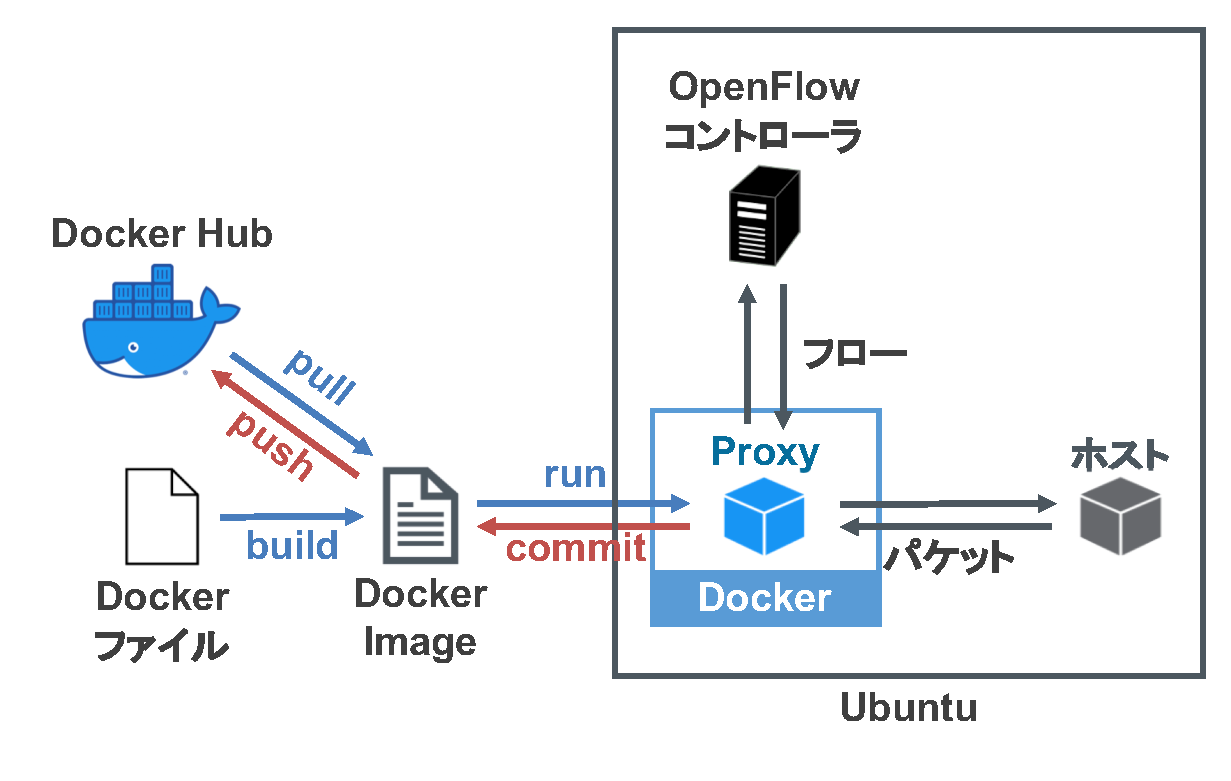
\includegraphics[width=\linewidth]{img/program.eps}
	\caption{実装環境の構成}
	\label{fig:program}
\end{figure}

\subsection{評価環境}
今回のシミュレーション実験においては,IoTデバイスや通信に関するログの収集・出力機能を実装し,セキュリティ対策として適用した.また,OpenFlowスイッチのイメージも取得し,OpenFlowによるフローチェックも行った.事前に2台のホストを設置した環境に,新たに1台ホストを追加し,そのホストが通信要求を行う環境を作成した.


\begin{figure*}[!tb]
	\centering
	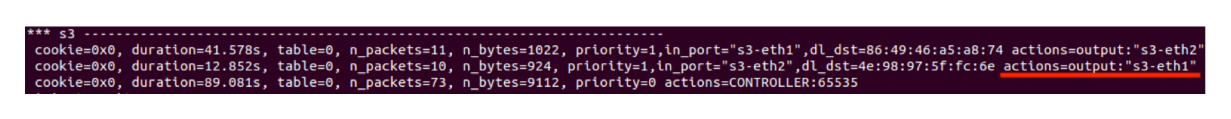
\includegraphics[width=\linewidth]{img/result_flow4v3.eps}
	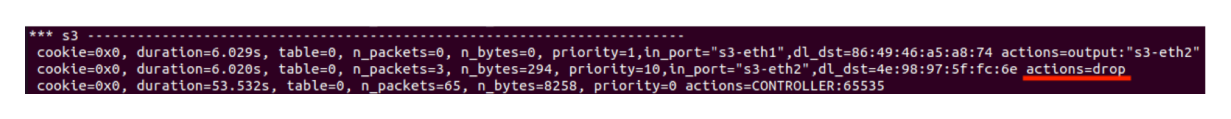
\includegraphics[width=\linewidth]{img/result_flow2v3.eps}
	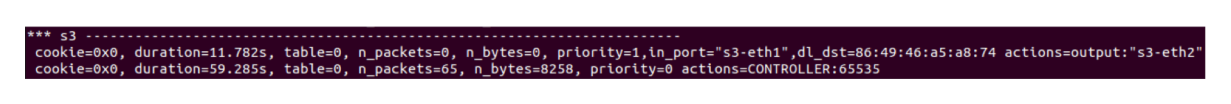
\includegraphics[width=\linewidth]{img/result_flow3v2.eps}
	\caption{登録済みのホストのフローテーブル(上),異常時のパケットをDrop処理するフローテーブル(中),その後のアクションが削除されたフローテーブル(下)}
	\label{fig:result1}
\end{figure*}

\section{結果と考察}
\subsection{評価結果}
登録済みのIoTデバイスから通信要求が来た場合,登録していないIoTデバイスや,通常の通信頻度と異なる等の異常の通信がなされている場合のフローテーブルの結果を図\ref{fig:result1}に示す.通常時は他のデバイスに対し,通信を許可するフローテーブルが作成されている.一方で,異常時はパケットをDrop処理するフローテーブルが作成されており,その後,そのフローテーブルが削除されていることがわかる.\par
また,セキュリティ対策を施した提案システムとセキュリティ対策を施してないシステムにおけるデバイス間通信の比較結果を図\ref{fig:result2}に示す.提案システムは,セキュリティ対策を施していないシステムにおける通信より,平均ラウンドトリップタイムが約1.06ms劣っていることがわかる.

\subsection{信頼性に関する考察}
ホームネットワーク内においても,IoTデバイス情報を基に,フローレベルで制御できることを示した.今回は,送信元IPアドレスや通信頻度の情報を用いたが,宛先IPアドレスやメッセージ情報を用いた追加のフロー制御を行うことで,更にセキュリティを高めることが可能である.\par
IoTデバイスを用いたシステムの安心安全を確保するための機能として,IPAによりIoT高信頼化機能が定義されている.また,IoT高信頼化要件として,開始,予防,検知,回復,終了の5つの局面に分けてそれぞれセキュリティ要件が定義されている\cite{IPA}.今回は前述の5つより,システム稼働中の局面である予防,検知,回復の3つにおける高信頼化要件に対し,提案システムの信頼性について考察する.

\begin{itemize}
	\item \underline{予防の局面における考察}\mbox{}\\
	      予防の局面での高信頼化要件は,稼働中の異常発生を未然に防止できることである.これに対応するIoT高信頼化機能としては,ログ収集機能,暗号化機能等があり,異常の予兆の把握や機能・資産の保護を実現する.提案システムを用いることで,リソース量の制限によりIoTデバイスに適用できない機能であっても適用可能となる.
	\item \underline{検知の局面における考察}\mbox{}\\
	      検知の局面での高信頼化要件は,稼働中の異常発生を早期に検知できることである.これに対応するIoT高信頼化機能としては,OpenFlowによるネットワーク監視機能,ログ収集機能があり,異常発生の検知や発生原因の特定を実現する.提案システムを用いることで,予防の局面同様,デバイスのリソース量に依存せず,要求機能を実現できる.また,Proxyは各IoTデバイスごとに作成するため,個々のデバイスに応じた検知対策を適用可能となる.
	\item \underline{回復の局面における考察}\mbox{}\\
	      回復の局面での高信頼化要件は,異常が発生した場合に稼働の維持や早期の復旧ができることである.ホームネットワークでは,様々なデバイスが相互通信を行うため,事前に予測していなかったインシデントが発生することが想定される.本提案システムにおいて,各セキュリティ対策はDocker HubからDocker Imageとして提供する.そのため,事前に作成したセキュリティ対策だけでなく,追加のセキュリティ対策も配布・適用することが容易である.従って,システムの早期復旧の実現が可能となる.
\end{itemize}

以上より,本提案システムは,システム稼働中の局面における高信頼化要件を満たしているため,信頼性を保っていることがわかる.

\begin{figure}[!tb]
	\centering
	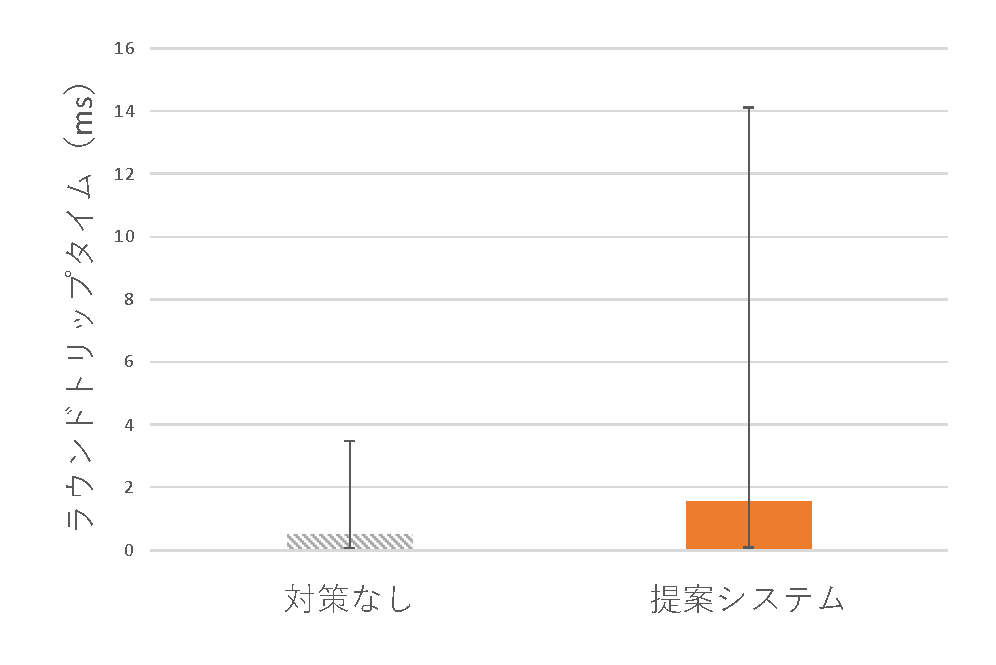
\includegraphics[width=\linewidth]{img/result.eps}
	\caption{デバイス間通信の平均ラウンドトリップタイム}
	\label{fig:result2}
\end{figure}

\subsection{通信性能に関する考察}
本提案システムは,セキュリティ対策なしの場合と比較し,約1.06msの遅延が発生した.これは,Dockerによって適用されたセキュリティ対策やOpenFlowによるフローチェックを行った際の負荷によるものである.しかし,スマートハウス等の領域では遅延許容度が高いとされている\cite{latency}ため,許容範囲内である.\par
今後,IoTデバイスが普及した際には,クラウドへの通信やデバイス間の通信が増加するため,帯域の輻輳や通信の干渉などの問題も発生すると予想される.そのため,より実環境に近い検証を行うために,デバイスの増加を想定した環境や,実機を用いた提案システムの性能検証を行う必要がある.

\section{まとめ}
本研究では,IoTのセキュリティ上のリスクにおいて,今後,ホームネットワーク内で閉じたデバイス間通信が多くなり,各IoTデバイスにおいてアクセス制御等の更なるセキュリティ対策を行う必要があることに注目した.
そこで,コンテナを用いたIoTデバイスへのセキュリティ対策の適用と,OpenFlowを用いたホームネットワーク監視を行うフレームワークの構築を提案した.提案システムでは,コンテナ上にProxyを作成し,ログ出力や暗号化,OpenFlowスイッチ等のセキュリティ対策をオフロードし,IoTデバイス間の通信を中継することで,本来IoTデバイスに適用したいセキュリティ対策を実現した.
そして,IoTデバイス間で閉じた通信を行うシミュレーション評価の比較を行い,提案システムはホームネットワークにおいてセキュリティ要件を保つことと,通信性能も許容範囲であることを示した.\par
今後は,ユーザの利便性を考慮し,オーケストレータ等を用いて,新しいIoTデバイスがホームネットワークに追加された際に,自動的にコンテナがProxyとして配備される仕組みを検討する.また,Raspberry Pi等の実機を用いて,より実環境に近い検証を行う予定である.

\begin{thebibliography}{10}
	\bibitem{security} 総務省:IoT・5Gセキュリティ総合対策2020,総務省(オンライン),
	\urlj{https://www.soumu.go.jp/\\main\_content/000698567.pdf}
	\refdatej{2022-03-28}.
	\bibitem{owasp} Ferrara, P., Mandal, A.K., Cortesi, A. and Spoto, F.: Static analysis for discovering IoT vulnerabilities, International Journal on Software Tools for Technology Transfer, Vol.23, No.1, pp.71-88(2021).
	\bibitem{camera} Abdalla, P.A. and Varol, C.: Testing IoT Security: The Case Study of an IP Camera, 2020 8th International Symposium on Digital Forensics and Security (ISDFS), pp.1-5(2020).
	\bibitem{disap} Serror, M., Henze, M., Hack, S., Schuba, M. and Wehrle, K.: Towards In-Network Security for Smart Homes, Proceedings of the 13th International Conference on Availability, Reliability and Security (ARES 2018), No.18, pp.1-8(2018).
	\bibitem{openflow} McKeown, N., Anderson, T., Balakrishnan, H., Parulkar, G., Peterson, L., Rexford, J., Shenker, S. and Turner, J.: OpenFlow: enabling innovation in campus networks, SIGCOMM Computer Communication Review, Vol.38, No.2, pp.69-74(2008).
	\bibitem{lowcost} Sivanathan, A., Sherratt, D., Gharakheili, H.H., Sivaraman, V. and Vishwanath, A.: Low-cost flow-based security solutions for smart-home IoT devices, 2016 IEEE International Conference on Advanced Networks and Telecommunications Systems (ANTS), pp.1-6(2016).
	\bibitem{d2d} Pawar, P. and Trivedi, A.: Device-to-Device Communication Based IoT System: Benefits and Challenges, IETE Technical Review, Vol.36, No.4, pp.362-374(2019).
	\bibitem{sover} Zhang, Z., Yu, T., Ma, X., Guan, Y., Moll, P. and Zhang, L.: Sovereign: Self-contained Smart Home with Data-centric Network and Security, IEEE Internet of Things Journal, pp.1-15(2022).
	\bibitem{IPA} 独立行政法人情報処理推進機構(IPA)技術本部 ソフトウェア高信頼化センター(SEC):「つながる世界の開発指針」の実践に向けた手引き[IoT高信頼化機能編],独立行政法人情報処理推進機構(IPA),pp.1-96(2017).
	\bibitem{latency} 総務省:スマートIoT推進戦略,総務省(オンライン),
	\urlj{https://www.soumu.go.jp/main\_content/\\000424359.pdf}
	\refdatej{2022-4-13}.

\end{thebibliography}

\end{document}
